% ==========================================================================
%  The Ten Commandments of Electrical Engineering  --  A1 portrait poster
%  Compile: just   (see justfile; latexmk settings in latexmkrc)
%  Needs: tikz, pgfplots, circuitikz, tcolorbox, mathpazo (all in TeX Live)
% ==========================================================================
\RequirePackage{fix-cm}
\documentclass{article}
\usepackage[paperwidth=594mm,paperheight=841mm,left=13mm,right=13mm,top=8mm,bottom=10mm]{geometry}
\usepackage[utf8]{inputenc}
\usepackage[T1]{fontenc}
\usepackage[sc]{mathpazo}          % Palatino text + math
\linespread{1.05}
\usepackage{amsmath,amssymb,bm}
\usepackage{xcolor}
\usepackage{tikz}
\usetikzlibrary{arrows.meta,positioning,calc,decorations.pathreplacing,patterns,shapes.symbols}
\usepackage{pgfplots}
\pgfplotsset{compat=1.16}
\usepackage[siunitx,american]{circuitikz}
\usepackage[most]{tcolorbox}
\tcbuselibrary{raster}

\pagestyle{empty}
\setlength{\parindent}{0pt}

% ---------------- palette ----------------
\definecolor{paper}{HTML}{F8F5EE}
\definecolor{ink}{HTML}{1E2430}
\definecolor{accent}{HTML}{1F4E79}
\definecolor{accentlt}{HTML}{6E93B5}
\definecolor{trap}{HTML}{9A3B2E}
\definecolor{muted}{HTML}{6B7280}
\definecolor{rule}{HTML}{B9C6D3}
\definecolor{good}{HTML}{3C7A4A}
\pagecolor{paper}
\color{ink}

% ---------------- sizes ----------------
\renewcommand{\normalsize}{\fontsize{17}{21}\selectfont}
\renewcommand{\small}{\fontsize{14}{17}\selectfont}
\renewcommand{\footnotesize}{\fontsize{12.5}{15}\selectfont}
\newcommand{\eqsize}{\fontsize{19}{23}\selectfont}
\newcommand{\mathbandsize}{\fontsize{19}{23}\selectfont}
\normalsize

\newcommand{\setdisplay}{%
  \setlength{\abovedisplayskip}{3pt}\setlength{\belowdisplayskip}{3pt}%
  \setlength{\abovedisplayshortskip}{3pt}\setlength{\belowdisplayshortskip}{3pt}}

% ---------------- equation group: a thin box holding equations that belong together
\newtcolorbox{eqgroup}[1][]{%
  enhanced, colback=white, colframe=rule, boxrule=0.7pt, arc=2.5mm,
  left=6pt, right=6pt, top=5pt, bottom=2pt, before skip=8pt, after skip=2pt,
  fontupper=\eqsize, before upper={\setdisplay},
  title={#1}, fonttitle=\footnotesize\scshape, coltitle=muted,
  attach boxed title to top left={xshift=4mm, yshift=-\tcboxedtitleheight/2},
  boxed title style={colback=white, colframe=white, boxrule=0pt, arc=0pt,
                     left=3pt, right=3pt, top=0pt, bottom=0pt}}
% single, ungrouped display equation
\newcommand{\eqn}[1]{{\eqsize\setdisplay\[#1\]}}
% minor / secondary equation (grey, smaller)
\newcommand{\minor}[1]{{\small\color{muted}\setdisplay\[#1\]}}

\newcommand{\trapicon}{\tikz[baseline=-0.15em]{%
  \fill[trap, rounded corners=1.2pt] (0,-0.12em) -- (1.15em,-0.12em) -- (0.575em,0.92em) -- cycle;
  \node[white, font=\bfseries\fontsize{11}{11}\selectfont, inner sep=0pt] at (0.575em,0.27em) {!};}}
\newcommand{\trap}[1]{{\centering\fontsize{14.5}{17.5}\selectfont\itshape\color{trap}#1\par}}

% ---------------- commandment box ----------------
% [#1] extra options, #2 roman numeral, #3 name, #4 the commandment, #5 unlocks (sits on the bottom border)
\newtcolorbox{commandment}[5][]{%
  enhanced, colback=white, colframe=accent, boxrule=1.4pt, arc=4mm,
  left=10pt, right=10pt, top=3pt, bottom=12pt,
  title={%
    \begin{tikzpicture}[baseline=(n.base)]
      \node[rounded corners=6mm, fill=white, text=accent, minimum height=12mm, minimum width=12mm, inner xsep=2.5mm, inner ysep=0pt,
            font=\fontsize{30}{30}\selectfont\bfseries] (n) {#2};
    \end{tikzpicture}\hspace{0.5em}%
    {\fontsize{26}{30}\selectfont\bfseries\itshape #4}},% #3 (topic name) kept in the source only, as a label
  colbacktitle=accent, coltitle=white,
  toptitle=2pt, bottomtitle=2pt, lefttitle=8pt, righttitle=12pt,
  segmentation hidden, space to upper, middle=1pt,
  overlay={\node[fill=white, draw=accent, line width=1.4pt, rounded corners=2.5mm,
                 inner xsep=9pt, inner ysep=5pt, font=\small, text=ink, anchor=center]
                 at (frame.south) {#5};},
  #1}

% two-part body: equations left, figure right
\newcommand{\body}[3][0.52]{%
  \begin{minipage}[c]{#1\linewidth}#2\end{minipage}\hfill
  \begin{minipage}[c]{\dimexpr\linewidth-#1\linewidth-6mm\relax}\centering #3\end{minipage}\par}

% common plot style
\pgfplotsset{posterplot/.style={
  width=120mm, height=46mm, axis lines=middle, axis line style={-{Latex[length=3mm]}, thick},
  tick style={draw=none}, ticklabel style={font=\small}, label style={font=\normalsize},
  every axis plot/.append style={line width=1.8pt}}}

\begin{document}
% ===================================================================== HEADER
\begin{minipage}[b]{0.61\linewidth}
  {\fontsize{28}{32}\selectfont\scshape\color{muted} The}\\[1mm]
  {\fontsize{96}{98}\selectfont\bfseries\scshape Ten Commandments}\\[4mm]
  {\fontsize{42}{48}\selectfont\itshape of Electrical Engineering}
\end{minipage}\hfill
\begin{minipage}[b]{0.38\linewidth}\raggedleft
% gutter note, read top to bottom along the right edge
\begin{tikzpicture}[remember picture, overlay]
  \node[rotate=-90, anchor=center, text=muted, font=\fontsize{14}{17}\selectfont\itshape]
    at ($(current page.east)+(-6.3mm,0mm)$)
    {No LLMs were harmed in the making of this poster.};
  \node[rotate=-90, anchor=center, text=muted, font=\fontsize{17}{20}\selectfont\itshape]
    at ($(current page.west)+(6.3mm,0mm)$)
    {Whoso can describe it, the machine will build. Whoso lacks the words: not even Saint Claudius can help.};
\end{tikzpicture}%
  {\fontsize{25}{30}\selectfont\color{muted}\itshape
   Whosoever studieth three years and knoweth not these ten,\\
   and whosoever teacheth and imparteth them not:\\
   \upshape\bfseries\color{trap} let both reconsider their life choices.}
\end{minipage}\par
\vspace{2mm}
{\color{accent}\rule{\linewidth}{2.5pt}}
\vspace{2mm}

% ===================================================================== CHAPTER i
\begin{tcolorbox}[enhanced, colback=white, colframe=ink, boxrule=1.6pt, arc=4mm,
  left=12pt, right=12pt, top=6pt, bottom=7pt,
  title={%
    {\fontsize{52}{52}\selectfont\bfseries\itshape i\kern0.04em}%
    {\fontsize{40}{44}\selectfont\bfseries\scshape n the Beginning was the Math}\hfill
    {\fontsize{22}{26}\selectfont\itshape $i^2=-1$\,; engineers call it $j$, for $i$ is betrothed.}},
  colbacktitle=ink, coltitle=white, toptitle=4pt, bottomtitle=4pt, lefttitle=10pt, righttitle=14pt]
\mathbandsize\setdisplay
\newcommand{\mathcol}[1]{\begin{minipage}[t]{0.327\linewidth}\vspace{0pt}#1\end{minipage}}
\begin{minipage}[t]{0.66\linewidth}
\mathcol{%
  \begin{eqgroup}[Euler: the most important line in the degree]
  \[ e^{j\theta}=\cos\theta+j\sin\theta \]
  \end{eqgroup}
  \begin{eqgroup}[Taylor: why linearisation works]
  \[ f(x_0+\Delta x)\approx f(x_0)+f'(x_0)\,\Delta x \]
  \end{eqgroup}
  \begin{eqgroup}[Decibels: logs turn products into sums]
  \[ G_{\mathrm{dB}}=10\log_{10}\frac{P_2}{P_1}=20\log_{10}\frac{V_2}{V_1} \]
  \end{eqgroup}
  \begin{eqgroup}[Parseval and Dirac]
  \[ \int|x(t)|^2dt=\int|X(f)|^2df \]
  \[ \int x(\tau)\,\delta(t-\tau)\,d\tau=x(t) \]
  \end{eqgroup}}\hfill
\mathcol{%
  \begin{eqgroup}[Linear systems and their modes]
  \[ A\mathbf x=\mathbf b \qquad A\mathbf v=\lambda\mathbf v \]
  \[ \det(A-\lambda I)=0 \]
  \end{eqgroup}
  \begin{eqgroup}[Transforms turn calculus into algebra]
  \[ X(\omega)=\int x(t)\,e^{-j\omega t}\,dt \]
  \[ \mathcal L\{\dot y\}=sY(s)-y(0) \]
  \[ X(z)=\sum_n x[n]\,z^{-n} \qquad z=e^{sT_s} \]
  \end{eqgroup}
  \begin{eqgroup}[Orthogonality: every coefficient is a projection]
  \[ c_k=\frac{\langle x,\varphi_k\rangle}{\langle\varphi_k,\varphi_k\rangle} \]
  \end{eqgroup}}\hfill
\mathcol{%
  \begin{eqgroup}[Divergence and Stokes]
  \[ \oint_S\mathbf F\cdot d\mathbf A=\int_V\nabla\cdot\mathbf F\,dV \]
  \[ \oint_C\mathbf F\cdot d\mathbf l=\int_S(\nabla\times\mathbf F)\cdot d\mathbf A \]
  \end{eqgroup}
  \begin{eqgroup}[Chance: Bayes, sums and the bell]
  \[ P(A\,|\,B)=\frac{P(B\,|\,A)\,P(A)}{P(B)} \]
  \[ \mathrm{Var}(X+Y)=\mathrm{Var}\,X+\mathrm{Var}\,Y \quad\text{(indep.)} \]
  \[ \bar x\ \sim\ \mathcal N\!\big(\mu,\ \sigma^2/n\big) \quad\text{(CLT)} \]
  \end{eqgroup}}
\end{minipage}\hfill
\begin{minipage}[t]{0.325\linewidth}\vspace{0pt}\centering
  \begin{eqgroup}[Second order: time and frequency]
  \[ \ddot y+2\zeta\omega_0\dot y+\omega_0^2y=\omega_0^2u \]
  \end{eqgroup}\vspace{1mm}
  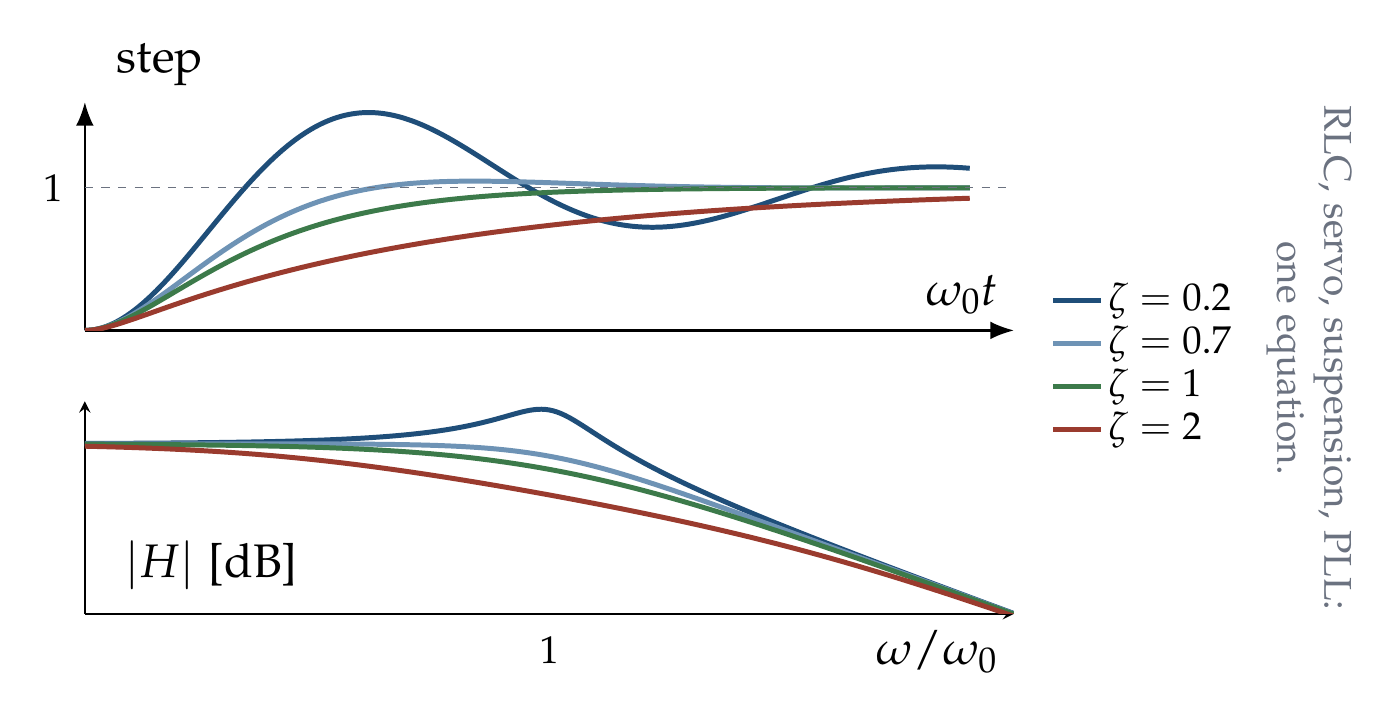
\begin{tikzpicture}
  \begin{axis}[posterplot, name=step, scale only axis, width=118mm, height=29mm, xmin=0, xmax=10.5, ymin=0, ymax=1.6,
     xlabel={$\omega_0 t$}, ylabel={step}, every axis y label/.style={at={(axis description cs:0,1)}, anchor=south west, xshift=2mm},
     xtick=\empty, ytick={1}, samples=140, domain=0:10,
     legend style={draw=none, fill=none, font=\small, at={(1.03,-0.15)}, anchor=west, row sep=-1pt}, legend cell align=left]
    \addplot[accent, smooth] {1-exp(-0.2*x)*(cos(deg(0.9798*x))+0.2041*sin(deg(0.9798*x)))};
    \addlegendentry{$\zeta=0.2$}
    \addplot[accentlt, smooth] {1-exp(-0.7*x)*(cos(deg(0.7141*x))+0.9802*sin(deg(0.7141*x)))};
    \addlegendentry{$\zeta=0.7$}
    \addplot[good, smooth] {1-(1+x)*exp(-x)};
    \addlegendentry{$\zeta=1$}
    \addplot[trap, smooth] {1+(-3.732*exp(-0.268*x)+0.268*exp(-3.732*x))/3.464};
    \addlegendentry{$\zeta=2$}
    \draw[muted, dashed, thin] (axis cs:0,1) -- (axis cs:10.5,1);
  \end{axis}
  \begin{semilogxaxis}[posterplot, name=bode, at={(step.south west)}, anchor=north west, yshift=-9mm, scale only axis, axis lines=left, width=118mm, height=27mm, xmin=0.1, xmax=10, ymin=-40, ymax=10,
     xlabel={$\omega/\omega_0$}, ylabel={$|H|$ [dB]},
     every axis y label/.style={at={(axis description cs:0,0)}, anchor=south west, xshift=3mm, yshift=1mm},
     every axis x label/.style={at={(axis description cs:1,0)}, anchor=north east},
     xtick={1}, xticklabels={$1$}, ytick=\empty, samples=120, domain=0.1:10]
    \addplot[accent, smooth] {-10*log10((1-x^2)^2+(0.4*x)^2)};
    \addplot[accentlt, smooth] {-10*log10((1-x^2)^2+(1.4*x)^2)};
    \addplot[good, smooth] {-10*log10((1-x^2)^2+(2*x)^2)};
    \addplot[trap, smooth] {-10*log10((1-x^2)^2+(4*x)^2)};
  \end{semilogxaxis}
  \node[rotate=-90, anchor=south, text=muted, font=\small, align=center]
    at ($(step.above north east)!0.5!(bode.below south east)+(30mm,0)$) {RLC, servo, suspension, PLL:\\ one equation.};
  \end{tikzpicture}
\end{minipage}

\vspace{6pt}
\trap{Behold, every signal hath two faces, time and frequency: cross over unto the side where the problem is easy, and ye shall find rest. \textbf{Prove all things:} check thy units, thy limits and thy signs; \textbf{hold fast that which is good.}}
\end{tcolorbox}

\vspace{6mm}

% ===================================================================== COMMANDMENTS
\noindent\begin{minipage}[t]{0.488\linewidth}
\begin{commandment}[equal height group=row1]{I}{Circuit laws}{Thou shalt conserve charge and energy.}{Nodal analysis $G\mathbf v=\mathbf i$ (what SPICE solves), mesh, superposition, dividers, loading.}
\body{%
  \begin{eqgroup}[Kirchhoff \& Ohm]
  \[ \textstyle\sum_{\text{node}} i=0 \qquad \sum_{\text{loop}} v=0 \qquad V=ZI \]
  \end{eqgroup}
  \begin{eqgroup}[Thévenin--Norton]
  \[ V_{Th}=V_{oc} \qquad Z_{Th}=\frac{V_{oc}}{I_{sc}} \]
  \[ \text{max power: } Z_L=Z_{Th}^{*} \]
  \end{eqgroup}}%
{%
  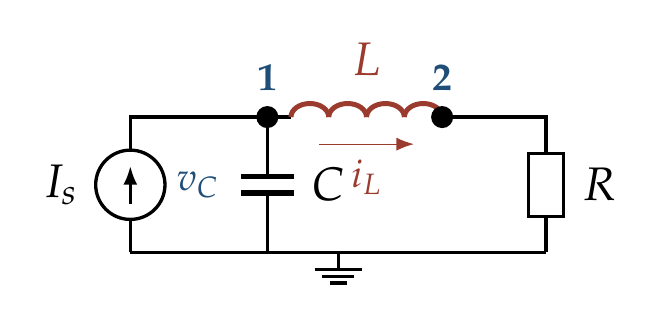
\begin{tikzpicture}[line width=1.2pt, x=12mm, y=8.6mm]
    % ground rail and top wires
    \draw (0,0) -- (4.4,0);
    \draw (0,0) -- (0,2) -- (1.7,2);
    \draw (3.3,2) -- (4.4,2) -- (4.4,0);
    % current source
    \draw[fill=white] (0,1) circle (4.4mm);
    \draw[-{Latex[length=2.4mm]}] (0,0.72) -- (0,1.28);
    \node[left=4.5mm] at (0,1) {$I_s$};
    % capacitor at node 1
    \draw (1.45,2) -- (1.45,1.12); \draw (1.45,0.88) -- (1.45,0);
    \draw[line width=2pt] (1.17,1.12) -- (1.73,1.12); \draw[line width=2pt] (1.17,0.88) -- (1.73,0.88);
    \node[right=3.5mm] at (1.45,1) {$C$};
    % inductor between node 1 and node 2 (highlighted)
        \foreach \i in {0,1,2,3} \draw[trap, line width=1.8pt] ({1.7+\i*0.4},2) arc (180:0:0.2);
    \node[trap, above=3mm] at (2.5,2) {$L$};
    \draw[-{Latex[length=2.2mm]}, trap, thin] (2.0,1.6) -- (3.0,1.6) node[midway, below, font=\small]{$i_L$};
    % resistor at node 2
    \node[draw, fill=white, minimum width=4.4mm, minimum height=8mm, inner sep=0pt] at (4.4,1) {};
    \node[right=2.5mm] at (4.4,1) {$R$};
    % nodes
    \fill (1.45,2) circle (1.4mm); \fill (3.3,2) circle (1.4mm);
    \node[font=\small\bfseries, text=accent, above=1.2mm] at (1.45,2) {1};
    \node[font=\small\bfseries, text=accent, above=1.2mm] at (3.3,2) {2};
    \node[font=\small, text=accent, anchor=east] at (1.12,1.0) {$v_C$};
    % ground
    \draw (2.2,0) -- (2.2,-0.25);
    \draw (1.95,-0.25) -- (2.45,-0.25); \draw (2.03,-0.35) -- (2.37,-0.35); \draw (2.11,-0.45) -- (2.29,-0.45);
  \end{tikzpicture}\\[1mm]
  {\fontsize{15}{18}\selectfont\arraycolsep=4pt
  $\displaystyle Y(s)=\begin{bmatrix} sC+\textcolor{trap}{\dfrac{1}{sL}} & \textcolor{trap}{-\dfrac{1}{sL}}\\[8pt] \textcolor{trap}{-\dfrac{1}{sL}} & \textcolor{trap}{\dfrac{1}{sL}}+\dfrac1R \end{bmatrix}$
  \hfill
  $\displaystyle A=\begin{bmatrix} 0 & -\dfrac1C\\[8pt] \dfrac1L & -\dfrac RL \end{bmatrix}$}\\[2mm]
  {\small\color{muted}$\det Y(s)=0$ and $\operatorname{eig}(A)$: the same poles.}}
\tcblower
\trap{\textbf{Leave no node floating.} Ask, and SPICE shall answer; but a node with no path to ground maketh the matrix singular.}
\end{commandment}
\end{minipage}\hfill%
\begin{minipage}[t]{0.488\linewidth}
\begin{commandment}[equal height group=row1]{II}{IQ \& phasors}{Thou shalt not forget the phase.}{AC analysis, Bode plots, modulation, I/Q receivers, Doppler radar.}
\body{%
  \begin{eqgroup}[A sinusoid is a complex number]
  \[ A\cos(\omega t+\varphi)=\mathrm{Re}\{\underbrace{Ae^{j\varphi}}_{I+jQ}\,e^{j\omega t}\} \]
  \end{eqgroup}
  \begin{eqgroup}[Calculus becomes algebra: $\tfrac{d}{dt}\to j\omega$]
  \[ Z_R=R \qquad Z_L=j\omega L \qquad Z_C=\frac{1}{j\omega C} \]
  \end{eqgroup}}%
{%
  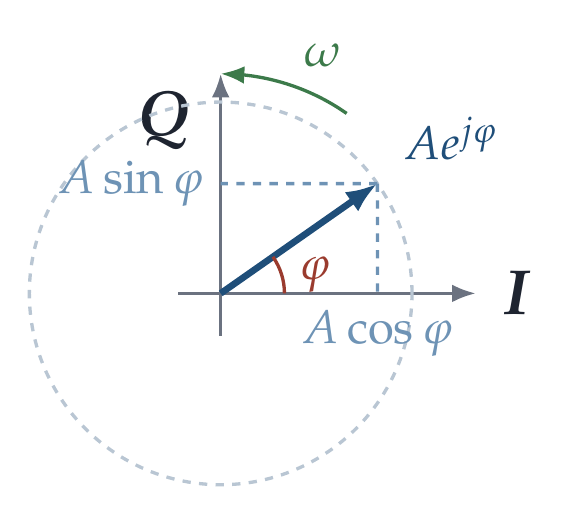
\begin{tikzpicture}[scale=0.9, line width=1.2pt]
    \draw[-{Latex[length=3mm]}, muted] (-0.6,0) -- (3.6,0) node[right=1mm, text=ink, font=\fontsize{23}{23}\selectfont]{$\boldsymbol I$};
    \draw[-{Latex[length=3mm]}, muted] (0,-0.6) -- (0,3.1) node[left=1.5mm, anchor=north east, text=ink, font=\fontsize{23}{23}\selectfont]{$\boldsymbol Q$};
    \draw[rule, dashed] (0,0) circle (2.7);
    \draw[-{Latex[length=4mm]}, accent, line width=2.4pt] (0,0) -- (35:2.7);
    \node[accent, anchor=south west] at (35:2.85) {$Ae^{j\varphi}$};
    \draw[dashed, accentlt] (35:2.7) -- (2.212,0) node[below]{$A\cos\varphi$};
    \draw[dashed, accentlt] (35:2.7) -- (0,1.549) node[left]{$A\sin\varphi$};
    \draw[trap] (0.9,0) arc (0:35:0.9) node[midway, right]{$\varphi$};
    \draw[-{Latex[length=3mm]}, good] (55:3.1) arc (55:90:3.1) node[midway, above right]{$\omega$};
      \end{tikzpicture}\\[1mm]
  {\small\color{muted}A QAM constellation is just points on this plane.}}
\tcblower
\trap{\textbf{A phasor hath neither beginning nor end:} one frequency, linear, for ever. For the moment of switching, go thou unto Laplace.}
\end{commandment}
\end{minipage}

\vspace{5mm plus 1fill}

\noindent\begin{minipage}[t]{0.488\linewidth}
\begin{commandment}[equal height group=row2]{III}{Convolution}{Thou shalt know thy impulse response.}{Transfer functions, FIR/IIR filters, FFT, equalisers; Fourier, Laplace and $Z$ transforms.}
\body{%
  \begin{eqgroup}[Time $\leftrightarrow$ frequency]
  \[ y(t)=\int x(\tau)\,h(t-\tau)\,d\tau \ \ \Longleftrightarrow\ \ Y=X\cdot H \]
  \end{eqgroup}
  \begin{eqgroup}[Causal \& stable]
  \[ h(t)=0 \text{ for } t<0 \qquad \text{poles: } \mathrm{Re}\,s<0,\ |z|<1 \]
  \end{eqgroup}}%
{%
  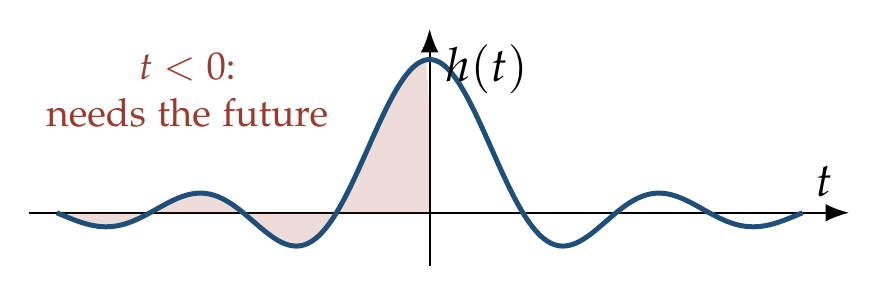
\begin{tikzpicture}
  \begin{axis}[posterplot, xmin=-4.3, xmax=4.5, ymin=-0.35, ymax=1.2, xlabel={$t$}, ylabel={$h(t)$},
      xtick=\empty, ytick=\empty, samples=200, domain=-4:4]
    \addplot[draw=none, fill=trap, fill opacity=0.18, domain=-4:0, samples=100] {sin(deg(pi*x))/(pi*x)} \closedcycle;
    \addplot[accent, smooth] {sin(deg(pi*x))/(pi*x)};
    \node[trap, font=\small, align=center] at (axis cs:-2.6,0.8) {$t<0$:\\needs the future};
  \end{axis}
  \end{tikzpicture}\\[1mm]
  {\small\color{muted}The ideal low-pass filter is a sinc: it can't be built in real time.}}
{\centering
  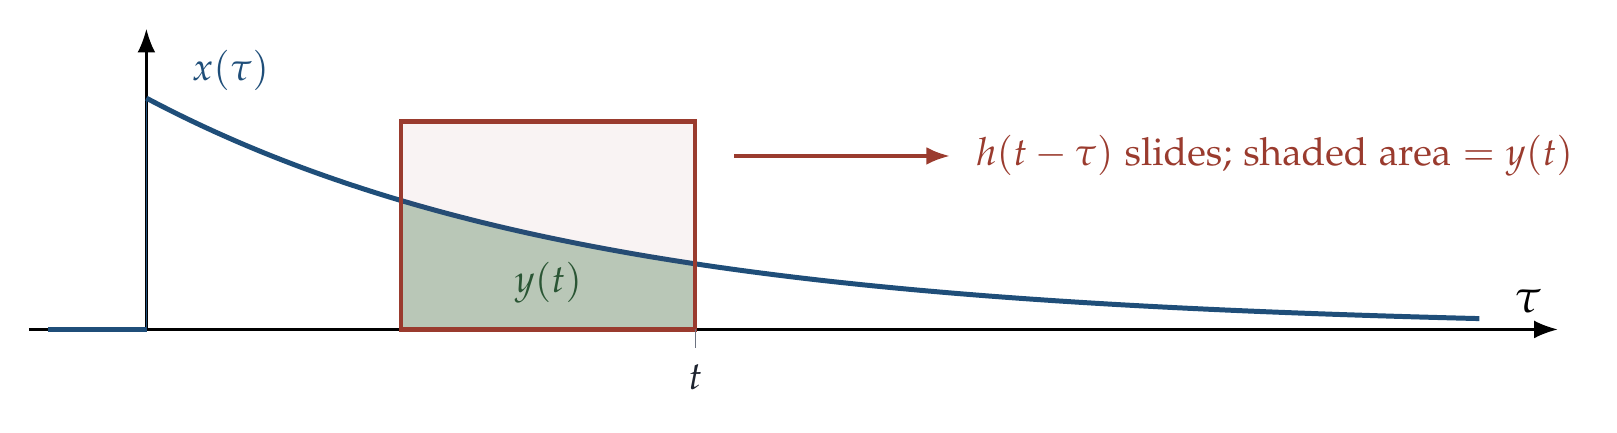
\begin{tikzpicture}
  \begin{axis}[posterplot, width=210mm, height=54mm, clip=false, xmin=-0.6, xmax=7.2, ymin=0, ymax=1.3,
      xlabel={$\tau$}, xtick=\empty, ytick=\empty, samples=120]
    \addplot[draw=none, fill=good, fill opacity=0.35, domain=1.3:2.8] {exp(-0.45*x)} \closedcycle;
    \addplot[accent, domain=0:6.8] {exp(-0.45*x)};
    \addplot[accent, domain=-0.5:0] {0};
    \draw[accent] (axis cs:0,0) -- (axis cs:0,1);
    \draw[trap, line width=1.6pt, fill=trap, fill opacity=0.06] (axis cs:1.3,0) rectangle (axis cs:2.8,0.9);
    \draw[-{Latex[length=3mm]}, trap, line width=1.4pt] (axis cs:3.0,0.75) -- (axis cs:4.1,0.75);
    \node[trap, font=\small, anchor=west] at (axis cs:4.15,0.75) {$h(t-\tau)$ slides; shaded area $=y(t)$};
    \node[accent, font=\small, anchor=west] at (axis cs:0.15,1.12) {$x(\tau)$};
    \node[good!70!black, font=\small] at (axis cs:2.05,0.2) {$y(t)$};
    \draw[muted, thin] (axis cs:2.8,0) -- (axis cs:2.8,-0.08) node[below, font=\small, text=ink]{$t$};
  \end{axis}
  \end{tikzpicture}\par}
\tcblower
\trap{\textbf{Sharp filters cost delay.} Narrow is the passband, and long the ringing thereof.}
\end{commandment}
\end{minipage}\hfill%
\begin{minipage}[t]{0.488\linewidth}
\begin{commandment}[equal height group=row2]{IV}{Shannon}{Thou shalt not sample below twice the bandwidth.}{ADCs, anti-aliasing filters, compression, error-correcting codes, adaptive QAM in Wi-Fi and 5G.}
\body{%
  \begin{eqgroup}[Sampling \& quantisation]
  \[ f_s>2B \qquad \sigma_q^2=\frac{\Delta^2}{12}\ \ \text{\small\color{muted}(6 dB per bit)} \]
  \end{eqgroup}
  \begin{eqgroup}[Capacity \& information]
  \[ C=B\log_2\!\Big(1+\frac{S}{N}\Big)\ \ \text{bit/s} \]
  \[ H=-\sum_i p_i\log_2 p_i \]
  \end{eqgroup}}%
{%
  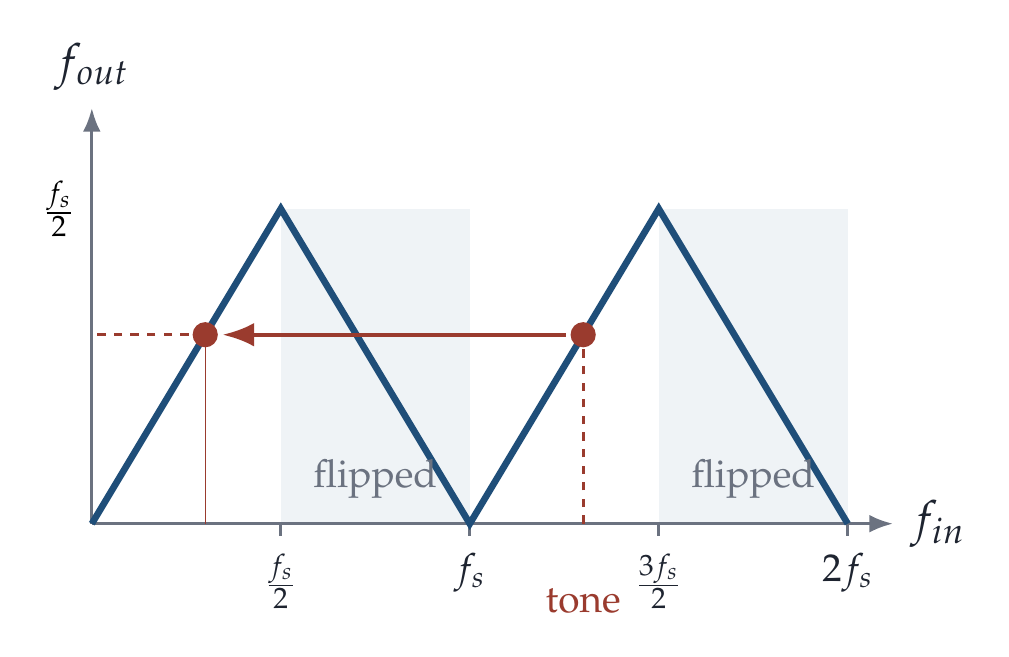
\begin{tikzpicture}[x=48mm, y=80mm, line width=1.2pt, >={Latex[length=3mm]}]
    % Nyquist zones (x in units of f_s, y in units of f_s)
    \foreach \z/\l in {0/1,1/2,2/3,3/4} {
      \pgfmathsetmacro{\xa}{\z*0.5}
      \ifodd\z \fill[accent!7] (\xa,0) rectangle ({\xa+0.5},0.5); \fi
    }
    % axes
    \draw[->, muted] (0,0) -- (2.12,0) node[right, text=ink]{$f_{in}$};
    \draw[->, muted] (0,0) -- (0,0.66) node[above, text=ink]{$f_{out}$};
    \foreach \x/\t in {0.5/{\tfrac{f_s}{2}},1/{f_s},1.5/{\tfrac{3f_s}{2}},2/{2f_s}}
      \draw[muted] (\x,0) -- (\x,-0.02) node[below, font=\small, text=ink]{$\t$};
    \node[left, font=\small] at (0,0.5) {$\tfrac{f_s}{2}$};
    % ping-pong
    \draw[accent, line width=2.4pt] (0,0) -- (0.5,0.5) -- (1,0) -- (1.5,0.5) -- (2,0);
    % example tone in zone 3 folds down
    \draw[trap, dashed] (1.3,0) -- (1.3,0.3);
    \draw[trap, dashed] (0.3,0.3) -- (0,0.3);
    \draw[trap, line width=1.6pt, -{Latex[length=4mm, width=3mm]}, shorten <=2.2mm, shorten >=2.2mm] (1.3,0.3) -- (0.3,0.3);
    \fill[trap] (1.3,0.3) circle (1.6mm);
    \fill[trap] (0.3,0.3) circle (1.6mm);
    \draw[trap, thin] (0.3,0) -- (0.3,0.3);
    \node[trap, font=\small, below] at (1.3,-0.075) {tone};
    \node[font=\small, muted, anchor=north] at (0.75,0.13) {flipped};
    \node[font=\small, muted, anchor=north] at (1.75,0.13) {flipped};
  \end{tikzpicture}\\[1mm]
  {\small\color{muted}Every frequency ping-pongs between $0$ and $f_s/2$; even zones arrive mirrored. Used on purpose, it is bandpass sampling.}}
\tcblower
\trap{\textbf{Aliasing is forever.} What the sampler hath joined together, let no filter put asunder: filter \emph{before} you sample.}
\end{commandment}
\end{minipage}

\vspace{5mm plus 1fill}

\noindent\begin{minipage}[t]{0.488\linewidth}
\begin{commandment}[equal height group=row3]{V}{State-space}{Thou shalt know thy state, and feed it.}{PID, pole placement, LQR, MPC, observers, Kalman filter, converter control loops.}
\body[0.42]{%
  \begin{eqgroup}[The system]
  \[ \left\{\begin{aligned} \dot{\mathbf x}&=A\mathbf x+B\mathbf u\\ \mathbf y&=C\mathbf x+D\mathbf u \end{aligned}\right. \]
  \end{eqgroup}
  \begin{eqgroup}[Feedback moves the poles]
  \[ \mathbf u=-K\mathbf x \ \Rightarrow\ \dot{\mathbf x}=(A-BK)\,\mathbf x \]
  \[ \text{stable} \iff \mathrm{Re}\,\lambda_i<0 \]
  \end{eqgroup}}%
{%
  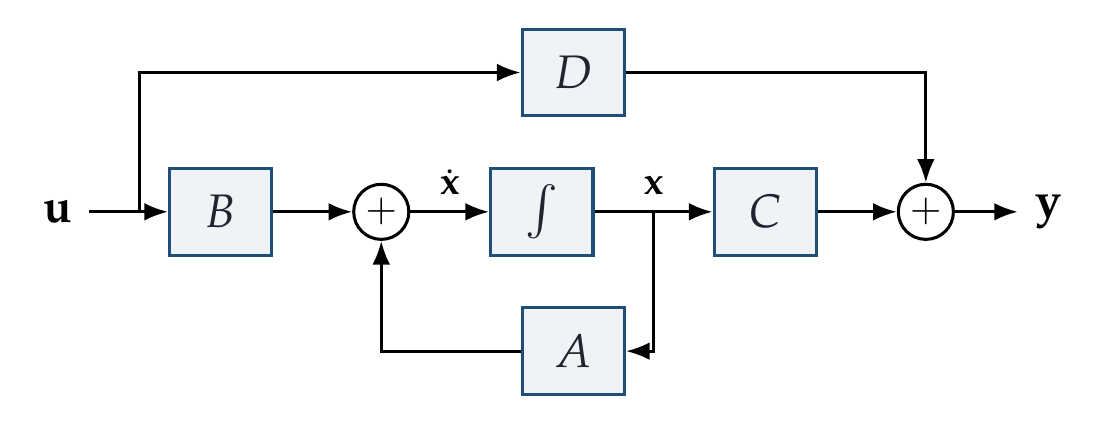
\begin{tikzpicture}[>={Latex[length=3mm]}, line width=1.1pt, node distance=13mm,
     blk/.style={draw, accent, fill=accent!7, minimum width=13mm, minimum height=11mm, font=\normalsize, text=ink},
     sum/.style={draw, circle, minimum size=7mm, inner sep=0pt, font=\small}]
    \node (u) {$\mathbf u$};
    \node[blk, right=10mm of u] (B) {$B$};
    \node[sum, right=10mm of B] (s1) {$+$};
    \node[blk, right=10mm of s1] (I) {$\int$};
    \node[blk, right=15mm of I] (C) {$C$};
    \node[sum, right=10mm of C] (s2) {$+$};
    \node[right=8mm of s2] (y) {$\mathbf y$};
    \node[blk, below=12mm of $(s1)!0.5!(C)$] (A) {$A$};
    \node[blk, above=12mm of $(B)!0.5!(s2)$] (D) {$D$};
    \draw[->] (u) -- (B); \draw[->] (B) -- (s1);
    \draw[->] (s1) -- node[above, font=\small]{$\dot{\mathbf x}$} (I);
    \draw[->] (I) -- node[above, font=\small]{$\mathbf x$} coordinate[pos=0.5](xm) (C);
    \draw[->] (C) -- (s2); \draw[->] (s2) -- (y);
    \draw[->] (xm) |- (A); \draw[->] (A) -| (s1);
    \draw[->] ($(u)!0.5!(B)$) |- (D); \draw[->] (D) -| (s2);
  \end{tikzpicture}\\[2mm]
  {\small\color{muted}Eigenvalues of $A$ are the poles of $H(s)$: same system, two views.}}
\tcblower
\trap{\textbf{Every linear model is local.} Stray far from thy operating point, and saturation shall find thee out.}
\end{commandment}
\end{minipage}\hfill%
\begin{minipage}[t]{0.488\linewidth}
\begin{commandment}[equal height group=row3]{VI}{Maxwell}{Thou shalt have no other equations.}{Circuits (the lumped limit), transmission lines beyond $\lambda/10$, antennas, motors, transformers, EMC.}
\body[0.615]{%
  \begin{eqgroup}[The four, and what thou calculatest with them]
  \newcommand{\mxname}[1]{\makebox[40mm][c]{\small\color{muted}#1}}%
  \[ \begin{alignedat}{3}
     \nabla\cdot\mathbf D&=\rho & \mxname{Gauss} && C&=\varepsilon A/d\\
     \nabla\cdot\mathbf B&=0 & \mxname{no monopoles} && \textstyle\sum\Phi&=0\\
     \nabla\times\mathbf E&=-\frac{\partial\mathbf B}{\partial t} & \mxname{Faraday} && v&=N\frac{d\Phi}{dt}\\
     \nabla\times\mathbf H&=\mathbf J+\frac{\partial\mathbf D}{\partial t} & \mxname{Ampère} && \textstyle\sum Hl&=NI
  \end{alignedat} \]
  \end{eqgroup}}%
{%
  {\fontsize{24}{28}\selectfont\bfseries\itshape\color{accent}\boldmath Let there be $\displaystyle c=\frac{1}{\sqrt{\mu_0\varepsilon_0}}$.}\\[2mm]
  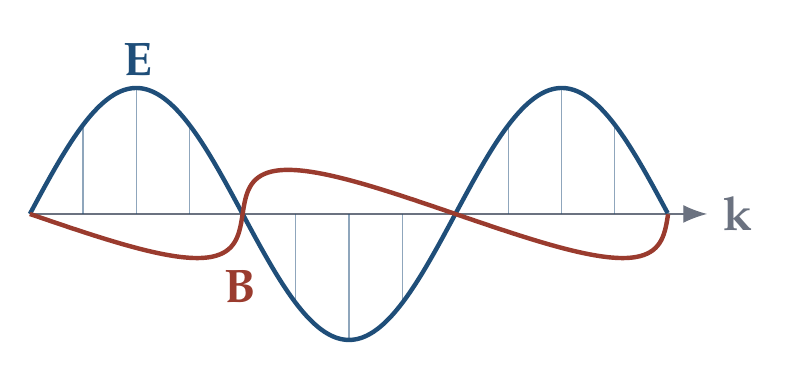
\begin{tikzpicture}[x=8.6mm, y=8mm, line width=1.6pt]
    \draw[-{Latex[length=3mm]}, muted, thin] (0,0) -- (10,0) node[right]{$\mathbf k$};
    \draw[accent, domain=0:9.42, samples=120, smooth] plot (\x, {2*sin(deg(\x*1))});
    \draw[trap, domain=0:9.42, samples=120, smooth] plot ({\x+0.9*sin(deg(\x))}, {-0.7*sin(deg(\x))});
    \foreach \t in {0.785, 1.571, 2.356, 3.927, 4.712, 5.498, 7.069, 7.854, 8.639}
      \draw[accent, thin, opacity=0.5] (\t,0) -- (\t,{2*sin(deg(\t))});
    \node[accent] at (1.6,2.45) {$\mathbf E$};
    \node[trap] at (3.1,-1.15) {$\mathbf B$};
  \end{tikzpicture}\\[1mm]
  {\small\color{muted}Faraday and Ampère feed each other, at $c$.}}
\tcblower
\trap{\textbf{Every wire is a component.} The trace the builder ignored is become a transmission line: 15\,cm per ns on a PCB.}
\end{commandment}
\end{minipage}

\vspace{5mm plus 1fill}

\noindent\begin{minipage}[t]{0.488\linewidth}
\begin{commandment}[equal height group=row4]{VII}{Power triangle}{Thou shalt pay for $S$.}{Three-phase, power-factor correction, grid control ($Q$ moves voltage, $P$ moves frequency), inverters.}
\body[0.40]{%
  \begin{eqgroup}[Complex power]
  \[ S=VI^{*}=P+jQ \]
  \[ \mathrm{PF}=\frac{P}{|S|}=\cos\varphi \]
  \end{eqgroup}
  \begin{eqgroup}[Three-phase]
  \[ P=\sqrt3\,V_{LL}I_L\cos\varphi \]
  \end{eqgroup}}%
{%
  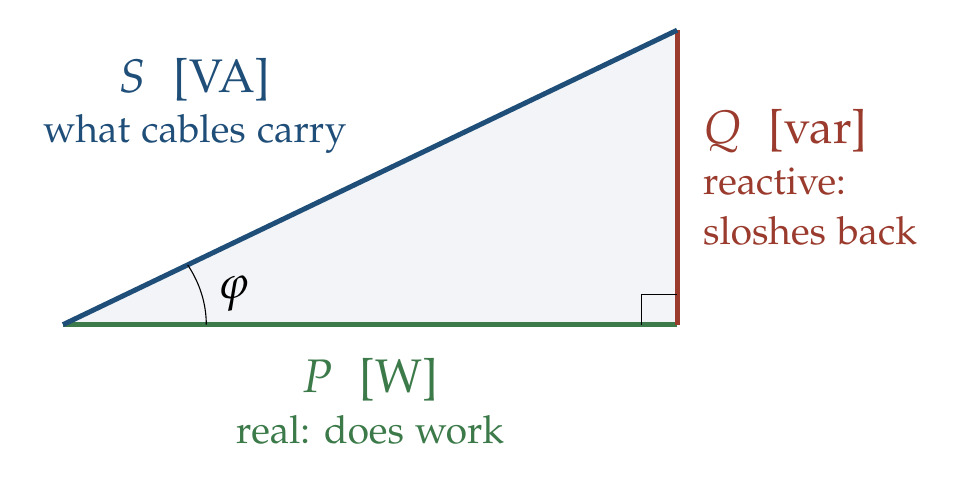
\begin{tikzpicture}[x=13mm, y=11mm, line width=1.8pt]
    \coordinate (O) at (0,0); \coordinate (P) at (6,0); \coordinate (S) at (6,3.4);
    \fill[accent!6] (O) -- (P) -- (S) -- cycle;
    \draw[good] (O) -- (P) node[midway, below=2mm, align=center]{$P$\ \ [W]\\[-1mm]{\small real: does work}};
    \draw[trap] (P) -- (S) node[midway, right=1mm, align=left]{$Q$\ \ [var]\\[-1mm]{\small reactive:}\\[-1mm]{\small sloshes back}};
    \draw[accent] (O) -- (S) node[midway, above left=1mm, align=center]{$S$\ \ [VA]\\[-1mm]{\small what cables carry}};
    \draw[thin] (5.65,0) -- (5.65,0.35) -- (6,0.35);
    \draw[thin] (1.4,0) arc (0:29.5:1.4) node[midway, right]{$\varphi$};
  \end{tikzpicture}}
\tcblower
\trap{\textbf{Render unto the cable its $|S|$:} $Q$ does no work, yet it heats the copper. With harmonics, $\cos\varphi$ is not the power factor.}
\end{commandment}
\end{minipage}\hfill%
\begin{minipage}[t]{0.488\linewidth}
\begin{commandment}[equal height group=row4]{VIII}{Probability \& noise}{Thou shalt not trust (a single measurement).}{Uncertainty budgets, bit error rate, receiver sensitivity, Friis noise figure, Kalman filtering.}
\body{%
  \begin{eqgroup}[Measurement (Student's $t$)]
  \[ \mu\in\bar x\pm t_{\alpha/2,\,n-1}\,\frac{s}{\sqrt n} \]
  \end{eqgroup}
  \begin{eqgroup}[Noise]
  \[ P_n=kTB \quad (-174\ \text{dBm/Hz}) \]
  \[ S_{yy}(f)=|H(f)|^2\,S_{xx}(f) \]
  \end{eqgroup}}%
{%
  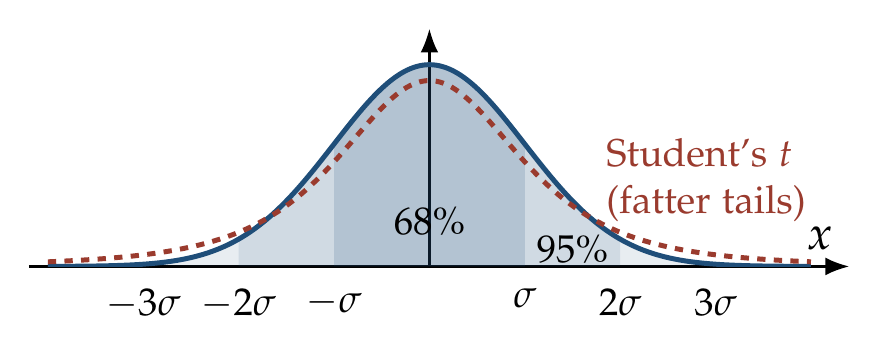
\begin{tikzpicture}
  \begin{axis}[posterplot, xmin=-4.2, xmax=4.4, ymin=0, ymax=0.47, xlabel={$x$}, ytick=\empty,
      xtick={-3,-2,-1,1,2,3}, xticklabels={$-3\sigma$,$-2\sigma$,$-\sigma$,$\sigma$,$2\sigma$,$3\sigma$},
      samples=120, domain=-4:4]
    \addplot[draw=none, fill=accent, fill opacity=0.10, domain=-3:3] {exp(-x^2/2)/sqrt(2*pi)} \closedcycle;
    \addplot[draw=none, fill=accent, fill opacity=0.12, domain=-2:2] {exp(-x^2/2)/sqrt(2*pi)} \closedcycle;
    \addplot[draw=none, fill=accent, fill opacity=0.16, domain=-1:1] {exp(-x^2/2)/sqrt(2*pi)} \closedcycle;
    \addplot[accent, smooth] {exp(-x^2/2)/sqrt(2*pi)};
    \addplot[trap, dashed, smooth] {0.3676*(1+x^2/3)^(-2)};
    \node[font=\small] at (axis cs:0,0.09) {$68\%$};
    \node[font=\small] at (axis cs:1.5,0.035) {$95\%$};
    \node[trap, font=\small, align=left] at (axis cs:2.9,0.17) {Student's $t$\\(fatter tails)};
  \end{axis}
  \end{tikzpicture}}
\tcblower
\trap{\textbf{Averaging cures only random error.} The systematic error ye have always with you.}
\end{commandment}
\end{minipage}

\vspace{5mm plus 1fill}

\noindent\begin{minipage}[t]{0.488\linewidth}
\begin{commandment}[equal height group=row5]{IX}{Semiconductors}{Honour thy thermal voltage.}{Amplifiers (gain $=g_mR$), op-amps, power MOSFETs and IGBTs, CMOS, LEDs, solar cells.}
\body{%
  \begin{eqgroup}[The junction]
  \[ I_D=I_S\big(e^{V_D/nV_T}-1\big) \qquad V_T=\frac{kT}{q}\approx26\ \text{mV} \]
  \end{eqgroup}
  \begin{eqgroup}[The transistor]
  \[ \text{BJT: } g_m=\frac{I_C}{V_T} \]
  \[ \text{MOSFET: } I_D=\tfrac12\mu C_{ox}\tfrac WL\,(V_{GS}-V_{th})^2 \]
  \end{eqgroup}}%
{%
  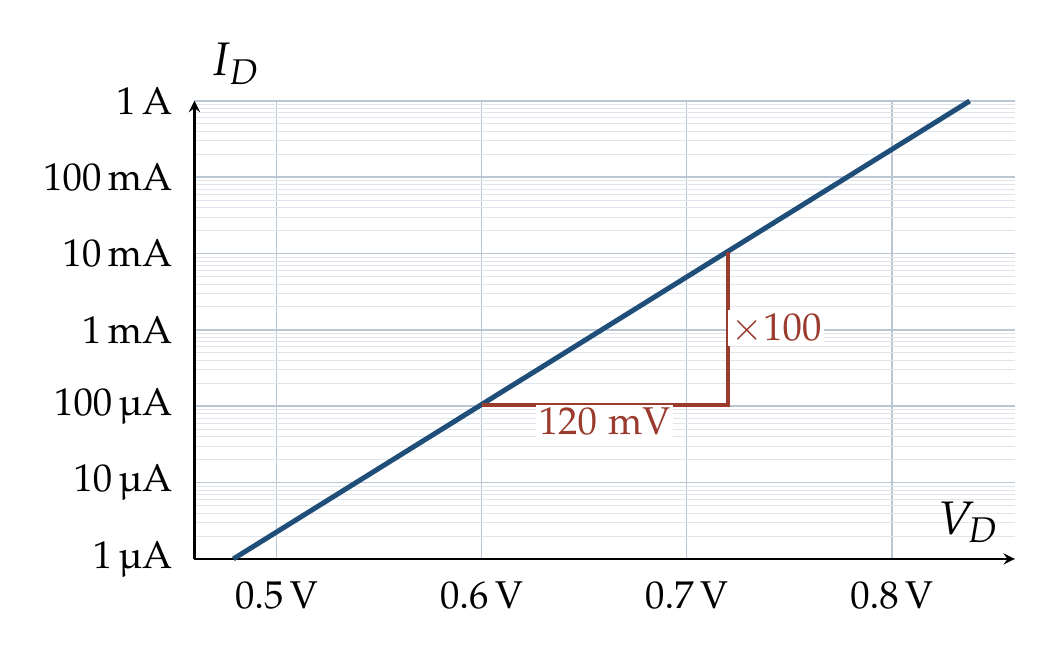
\begin{tikzpicture}
  \begin{axis}[posterplot, height=74mm, clip=false, axis lines=left, ymode=log, log basis y=10,
      xmin=0.46, xmax=0.86, ymin=1e-6, ymax=1,
      xlabel={$V_D$}, ylabel={},
      xtick={0.5,0.6,0.7,0.8}, xticklabels={0.5\,V,0.6\,V,0.7\,V,0.8\,V},
      ytick={1e-6,1e-5,1e-4,1e-3,1e-2,1e-1,1},
      yticklabels={1\,\textmu A,10\,\textmu A,100\,\textmu A,1\,mA,10\,mA,100\,mA,1\,A},
      minor ytick={2e-6,3e-6,4e-6,5e-6,6e-6,7e-6,8e-6,9e-6,
                   2e-5,3e-5,4e-5,5e-5,6e-5,7e-5,8e-5,9e-5,
                   2e-4,3e-4,4e-4,5e-4,6e-4,7e-4,8e-4,9e-4,
                   2e-3,3e-3,4e-3,5e-3,6e-3,7e-3,8e-3,9e-3,
                   2e-2,3e-2,4e-2,5e-2,6e-2,7e-2,8e-2,9e-2,
                   0.2,0.3,0.4,0.5,0.6,0.7,0.8,0.9},
      ymajorgrids, yminorgrids, xmajorgrids,
      major grid style={rule, line width=0.6pt}, minor grid style={rule!45, line width=0.3pt},
      samples=60, domain=0.479:0.838]
    \addplot[accent] {1e-14*exp(x/0.026)};
    \node[anchor=south west, font=\normalsize] at (rel axis cs:0,1) {$I_D$};
    \draw[trap, line width=1.4pt] (axis cs:0.60,1.05e-4) -- (axis cs:0.72,1.05e-4) -- (axis cs:0.72,1.05e-2);
    \node[trap, font=\small, below, fill=white, inner sep=1pt] at (axis cs:0.66,1.05e-4) {120 mV};
    \node[trap, font=\small, right, fill=white, inner sep=1pt] at (axis cs:0.72,1.05e-3) {$\times100$};
  \end{axis}
  \end{tikzpicture}\\[1mm]
  {\small\color{muted}On log paper the exponential is a straight line: $\times10$ per 60\,mV, set by $V_T$.}}
\tcblower
\trap{\textbf{Beware thermal runaway.} Heat begat current, and current begat heat ($V_{BE}$ falls 2\,mV/\textdegree C): emitter resistors break the line.}
\end{commandment}
\end{minipage}\hfill%
\begin{minipage}[t]{0.488\linewidth}
\begin{commandment}[equal height group=row5]{X}{Logic \& timing}{Thou shalt not covet thy neighbour's clock.}{State machines, FPGAs, CPUs, embedded systems.}
\centering
\begin{minipage}[c]{0.92\linewidth}\centering
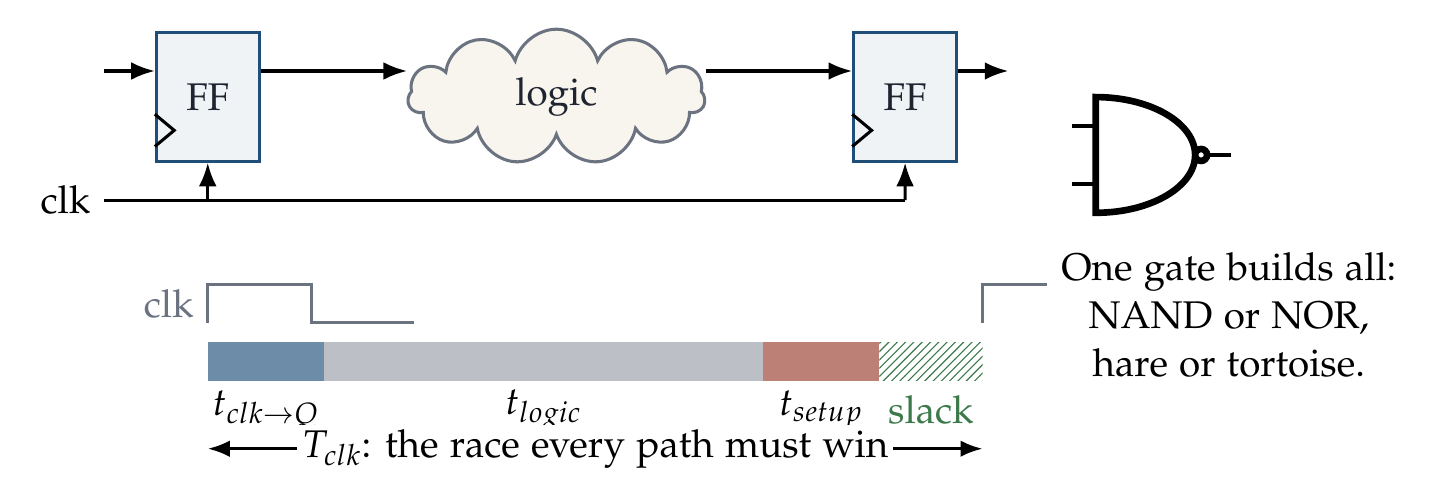
\begin{tikzpicture}[scale=0.82, transform shape, >={Latex[length=3mm]}, line width=1.1pt,
   ff/.style={draw, accent, fill=accent!7, minimum width=16mm, minimum height=20mm, text=ink, font=\normalsize}]
  % datapath
  \node[ff] (f1) at (0,0) {FF};
  \node[cloud, draw, muted, fill=paper, cloud puffs=11, aspect=2.4, minimum width=46mm, minimum height=20mm, text=ink, font=\normalsize] (L) at (5.4,0) {logic};
  \node[ff] (f2) at (10.8,0) {FF};
  \draw[->] (-1.6,0.4) -- (f1.west |- 0,0.4);
  \draw[->] (f1.east |- 0,0.4) -- (L.west |- 0,0.4);
  \draw[->] (L.east |- 0,0.4) -- (f2.west |- 0,0.4);
  \draw[->] (f2.east |- 0,0.4) -- (12.4,0.4);
  \foreach \f in {f1,f2} \draw ($(\f.south west)+(0,0.25)$) -- ($(\f.south west)+(0.3,0.5)$) -- ($(\f.south west)+(0,0.75)$);
  \draw (-1.6,-1.6) node[left, font=\normalsize]{clk} -- (10.8,-1.6);
  \draw[->] (0,-1.6) -- (f1.south); \draw[->] (10.8,-1.6) -- (f2.south);
  % timing bar
  \begin{scope}[yshift=-3.5cm]
    \draw[muted] (0,0) -- (0,0.6) -- (1.6,0.6) -- (1.6,0) -- (3.2,0);
    \draw[muted] (12.0,0) -- (12.0,0.6) -- (13.0,0.6);
    \node[muted, font=\normalsize, left] at (0,0.3) {clk};
    \fill[accent!65]    (0,-0.9)  rectangle (1.8,-0.3);
    \fill[muted!45]     (1.8,-0.9) rectangle (8.6,-0.3);
    \fill[trap!65]      (8.6,-0.9) rectangle (10.4,-0.3);
    \fill[pattern=north east lines, pattern color=good] (10.4,-0.9) rectangle (12.0,-0.3);
    \node[font=\normalsize] at (0.9,-1.35) {$t_{clk\to Q}$};
    \node[font=\normalsize] at (5.2,-1.35) {$t_{logic}$};
    \node[font=\normalsize] at (9.5,-1.35) {$t_{setup}$};
    \node[font=\normalsize, good] at (11.2,-1.35) {slack};
    \draw[{Latex}-{Latex}] (0,-1.95) -- (12.0,-1.95) node[midway, fill=white, inner sep=2pt, font=\normalsize]{$T_{clk}$: the race every path must win};
  \end{scope}
  % NAND
  \begin{scope}[xshift=15.6cm, yshift=-0.9cm]
    \draw (0,0) node[nand port, scale=1.6, line width=1.2pt] (n) {};
    \node[font=\normalsize, align=center, below=4mm of n, xshift=12mm] {One gate builds all:\\NAND or NOR,\\hare or tortoise.};
  \end{scope}
\end{tikzpicture}
\end{minipage}\hfill
\begin{minipage}[c]{0.07\linewidth}\centering
\rotatebox[origin=c]{-90}{\begin{tabular}{@{}c@{}}{\itshape\color{muted}``Every idiot can count to one.''}\\[1pt]{\small\color{muted}--- attrib.\ Bob Widlar}\end{tabular}}
\end{minipage}\\[1mm]
{\eqsize $T_{clk}\ \ge\ t_{clk\to Q}+t_{logic}+t_{setup}$ \qquad $\mathrm{MTBF}=\dfrac{e^{\,t_r/\tau}}{T_0\,f_{clk}\,f_{data}}$}\par\vspace{6pt}
\raggedright
\tcblower
\trap{\textbf{Synchronise every crossing.} No flip-flop can serve two clocks: pass foreign signals through two flip-flops in a row.}
\end{commandment}
\end{minipage}




\end{document}
